\chapter{Señales a través del canal con fallas}
En este apéndice mostramos las salidas del banco de filtro y de los posteriores bloques RMS. Analizamos las señales que codifican a todos los números del teclado; con estas codificaciones abarcamos todas las áreas del espectro \gls{dtfm}. Recordar que estas simulaciones son para el canal amplificado en 3.

\pagebreak

\section{Número 1: 697 [Hz] + 1209 [Hz]}
\label{sec:signal_1}
\begin{figure}[H]
  \centering
  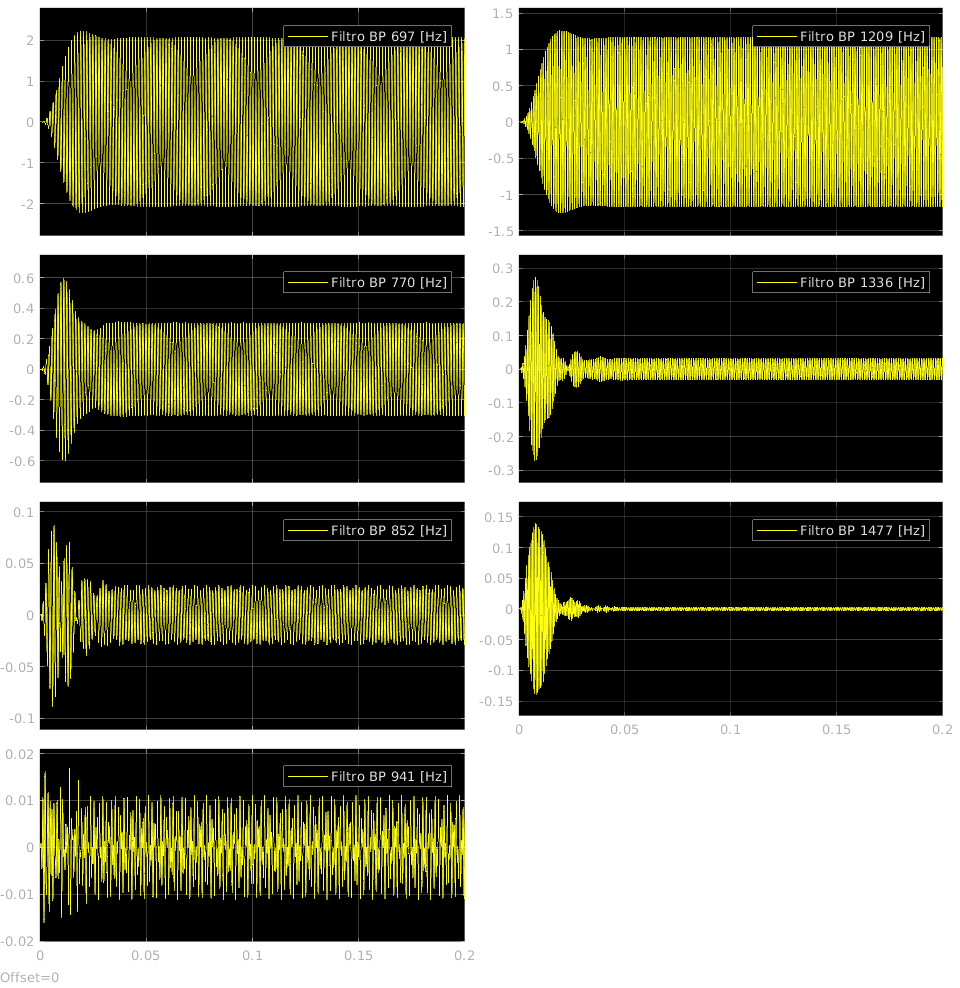
\includegraphics[width=\linewidth]{images/simulacion/fallas/bank/1.png}
  \caption{Señales en el Banco de Filtro}
  \label{fig:num_1_bank}
\end{figure}

\begin{figure}[H]
  \centering
  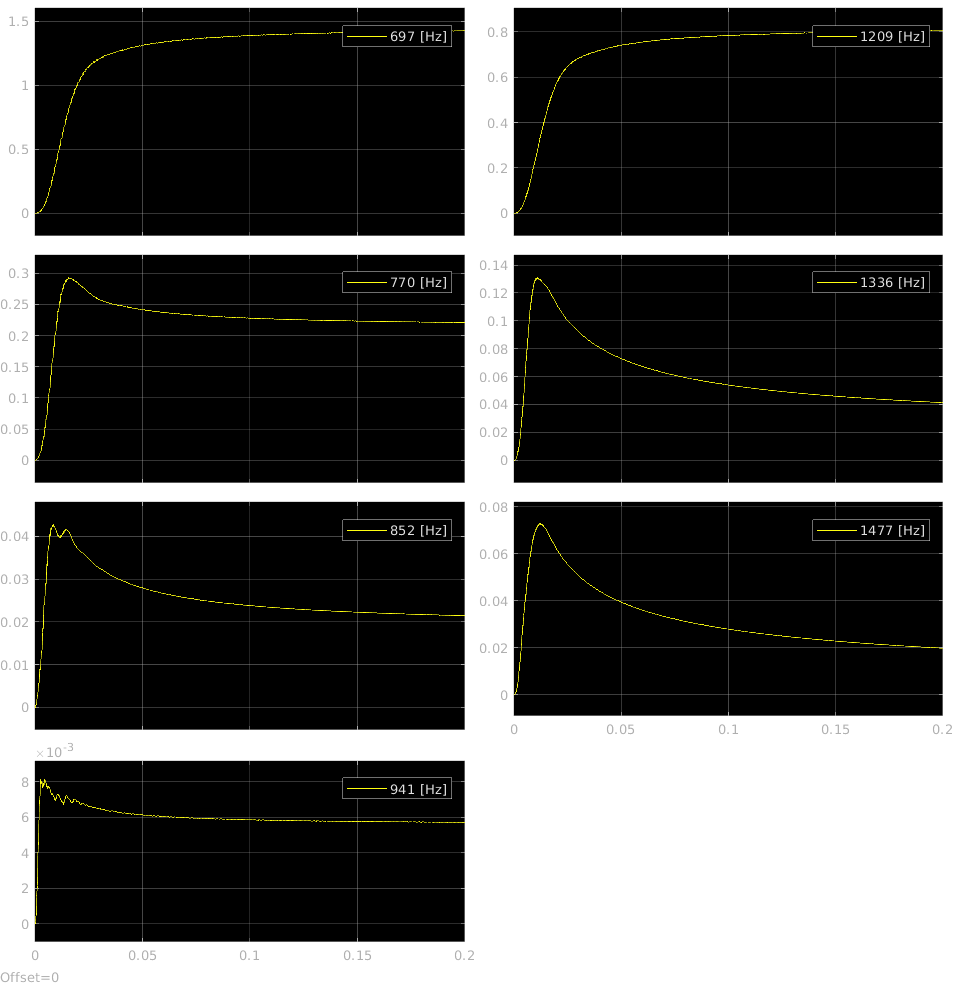
\includegraphics[width=\linewidth]{images/simulacion/fallas/rms/1.png}
  \caption{Valor Eficaz de las salida del Banco de Filtros }
  \label{fig:num_1_rms}
\end{figure}

Debido a que el valor eficaz de la señal del filtro de 1209 [Hz] es menor a 1, esta se toma como 0 para la compuerta lógica. En consecuencia, no se reconoce la activación de la Tecla 1.

% ******************************************************* %

\section{Número 2: 697 [Hz] + 1336 [Hz]}
\label{sec:signal_2}
\begin{figure}[H]
  \centering
  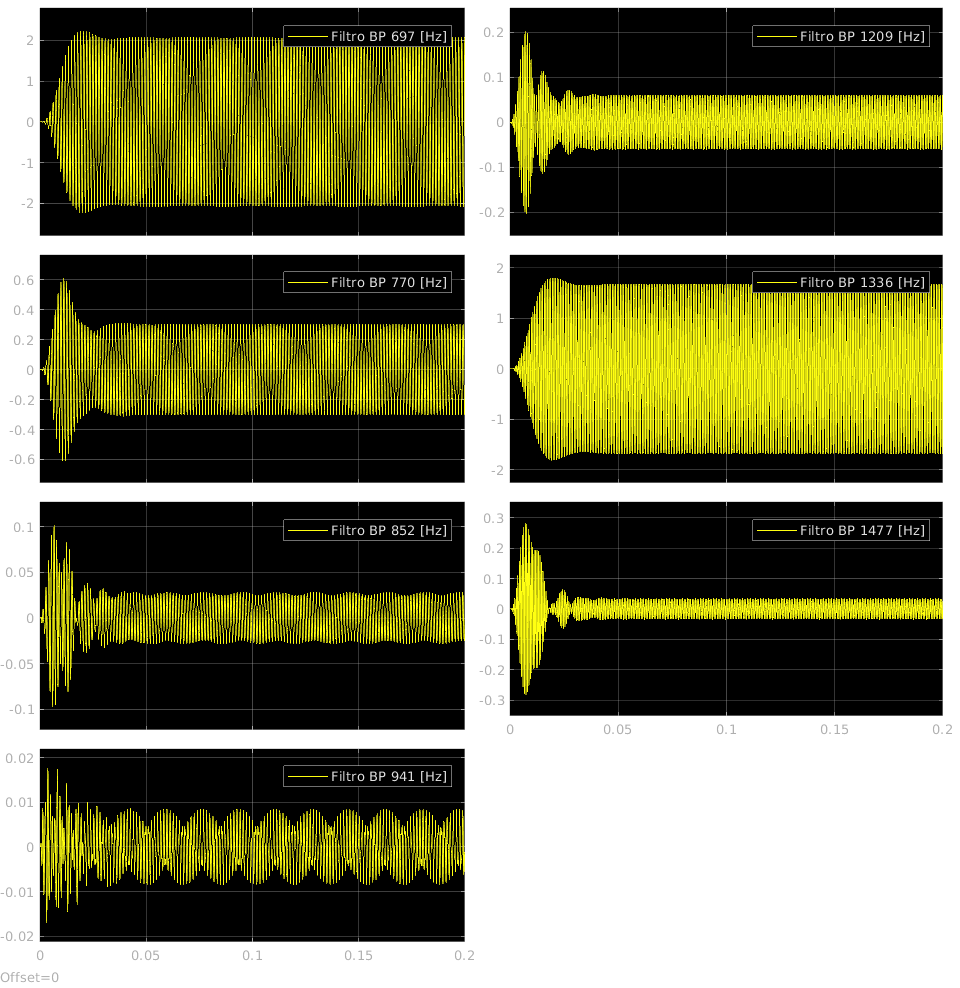
\includegraphics[width=\linewidth]{images/simulacion/fallas/bank/2.png}
  \caption{Señales en el Banco de Filtro}
  \label{fig:num_2_bank}
\end{figure}

\begin{figure}[H]
  \centering
  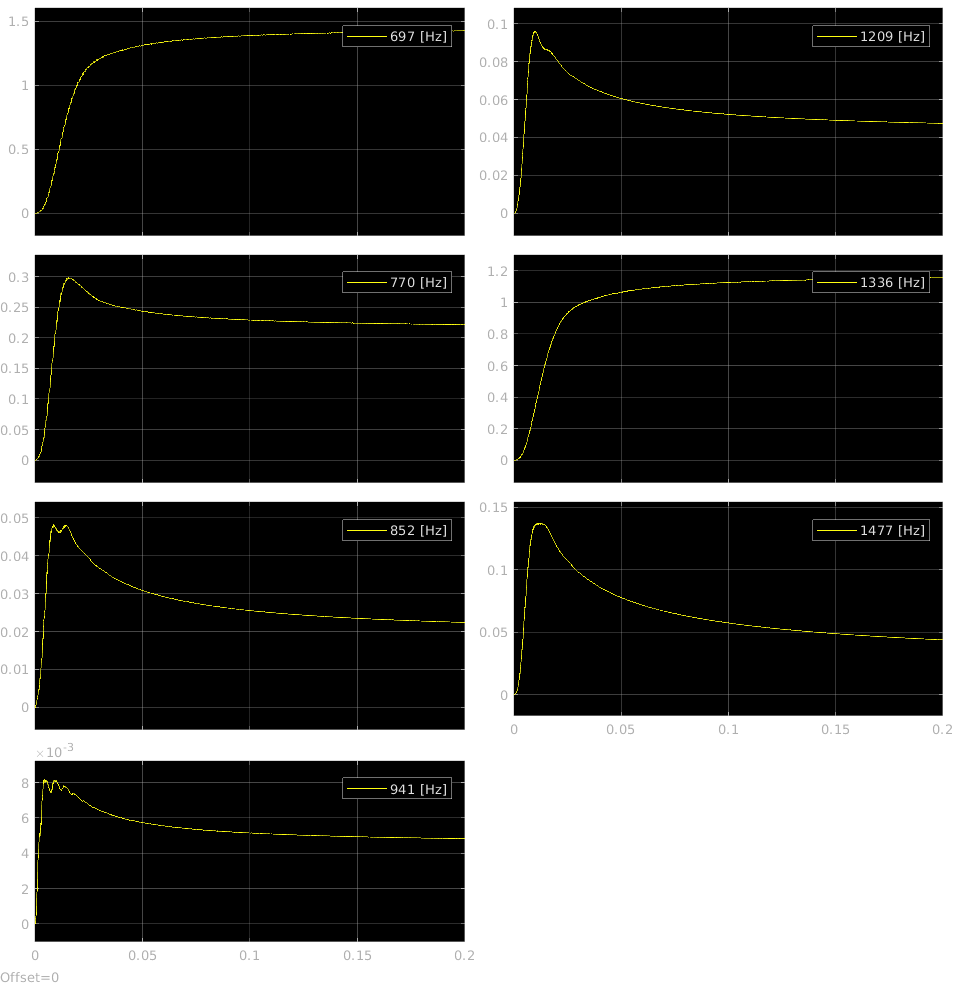
\includegraphics[width=\linewidth]{images/simulacion/fallas/rms/2.png}
  \caption{Valor Eficaz de las salida del Banco de Filtros }
  \label{fig:num_2_rms}
\end{figure}

Ya que ambos valores eficaces de las señales que codifican la Tecla 2 son mayores a 1, se reconoce la activación de la misma.

% ******************************************************* %

\section{Número 3: 697 [Hz] + 1477 [Hz]}
\label{sec:signal_3}
\begin{figure}[H]
  \centering
  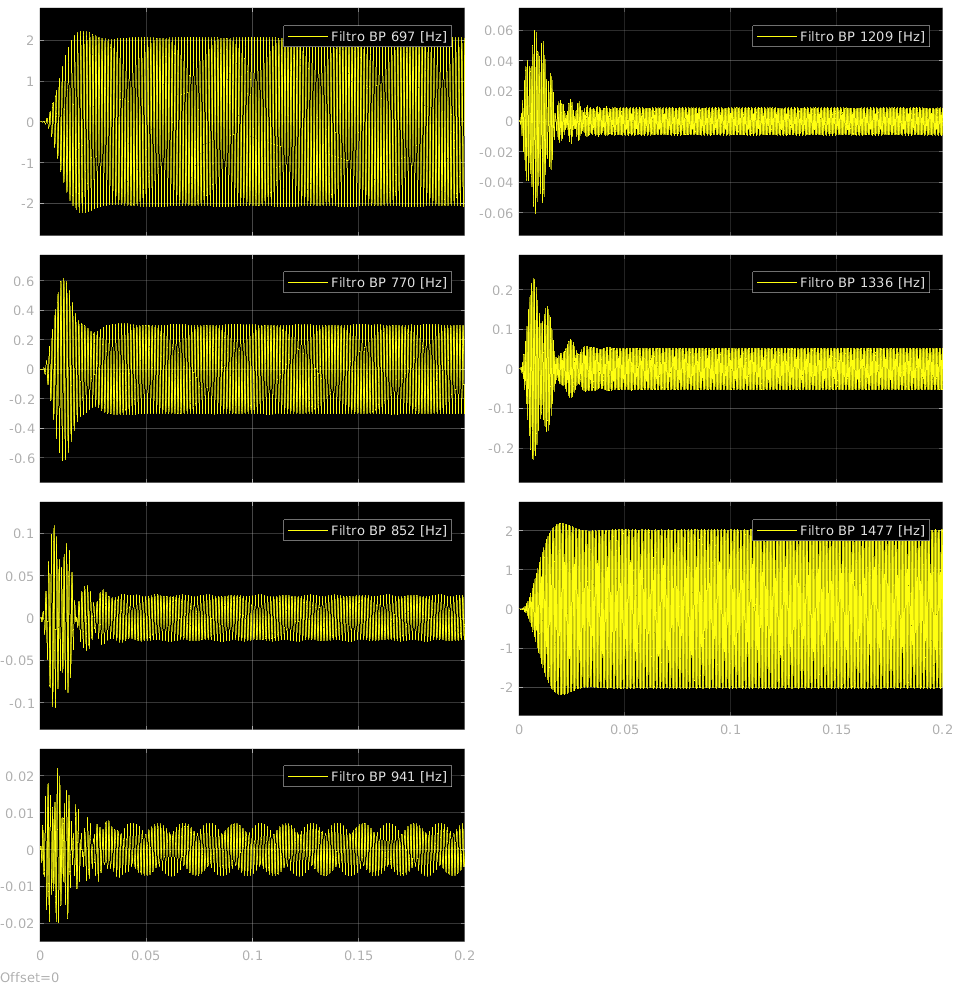
\includegraphics[width=\linewidth]{images/simulacion/fallas/bank/3.png}
  \caption{Señales en el Banco de Filtro}
  \label{fig:num_3_bank}
\end{figure}

\begin{figure}[H]
  \centering
  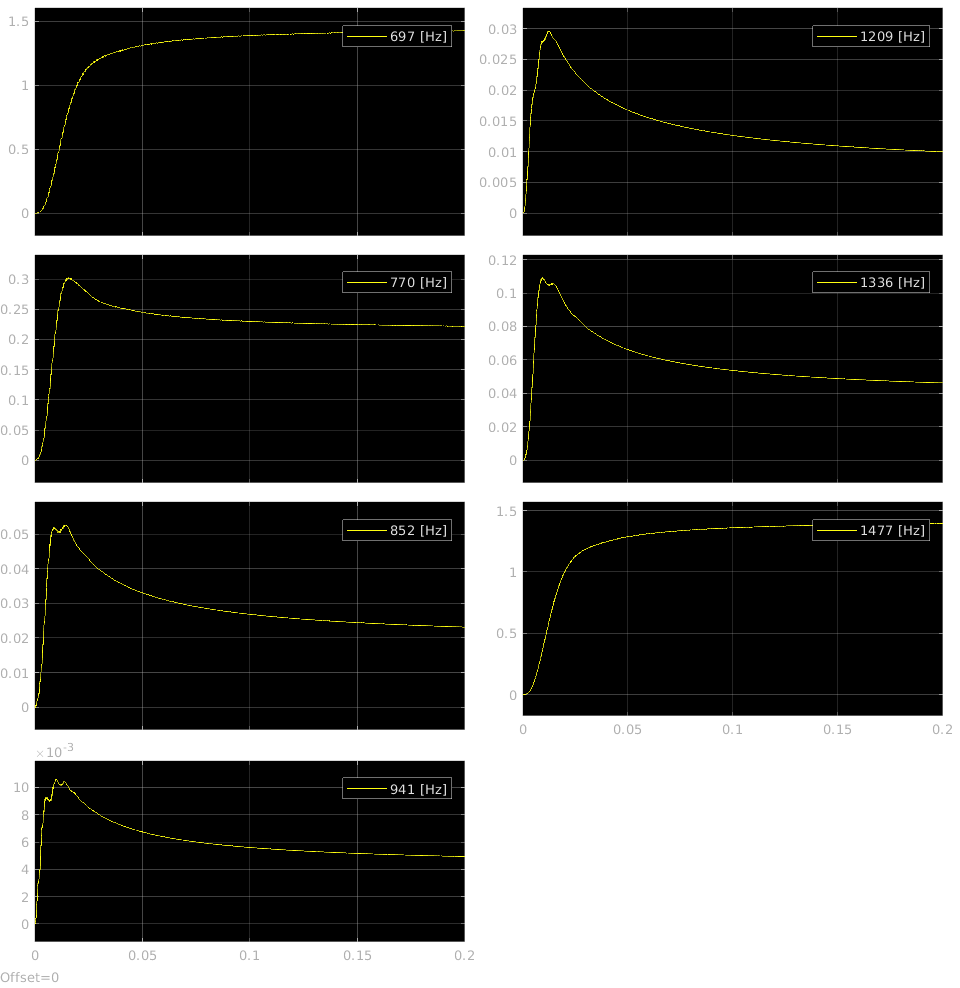
\includegraphics[width=\linewidth]{images/simulacion/fallas/rms/3.png}
  \caption{Valor Eficaz de las salida del Banco de Filtros }
  \label{fig:num_3_rms}
\end{figure}

Ya que ambos valores eficaces de las señales que codifican la Tecla 3 son mayores a 1, se reconoce la activación de la misma.

% ******************************************************* %

\section{Número 4: 770 [Hz] + 1336 [Hz]}
\label{sec:signal_4}
\begin{figure}[H]
  \centering
  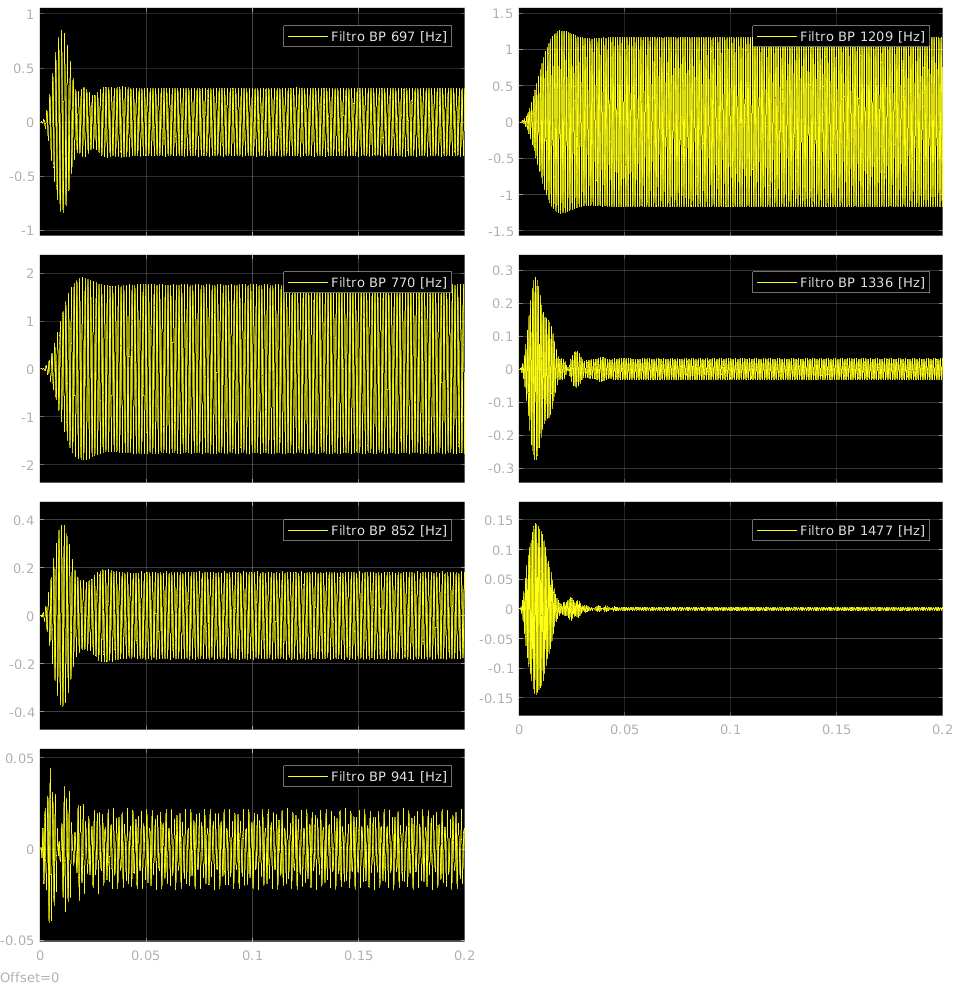
\includegraphics[width=\linewidth]{images/simulacion/fallas/bank/4.png}
  \caption{Señales en el Banco de Filtro}
  \label{fig:num_4_bank}
\end{figure}

\begin{figure}[H]
  \centering
  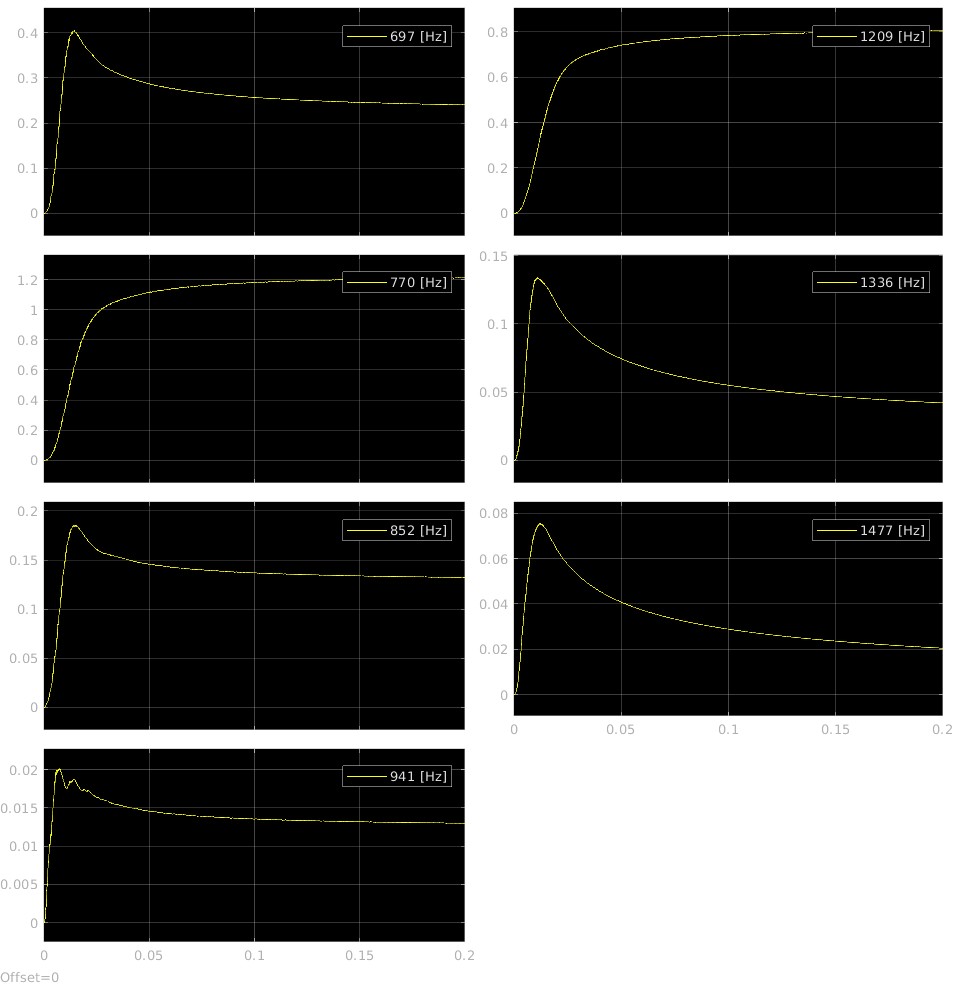
\includegraphics[width=\linewidth]{images/simulacion/fallas/rms/4.png}
  \caption{Valor Eficaz de las salida del Banco de Filtros }
  \label{fig:num_4_rms}
\end{figure}

Debido a que el valor eficaz de la señal del filtro de 1209 [Hz] es menor a 1, esta se toma como 0 para la compuerta lógica. En consecuencia, no se reconoce la activación de la Tecla 4.

% ******************************************************* %

\section{Número 5: 770 [Hz] + 1336 [Hz]}
\label{sec:signal_5}
\begin{figure}[H]
  \centering
  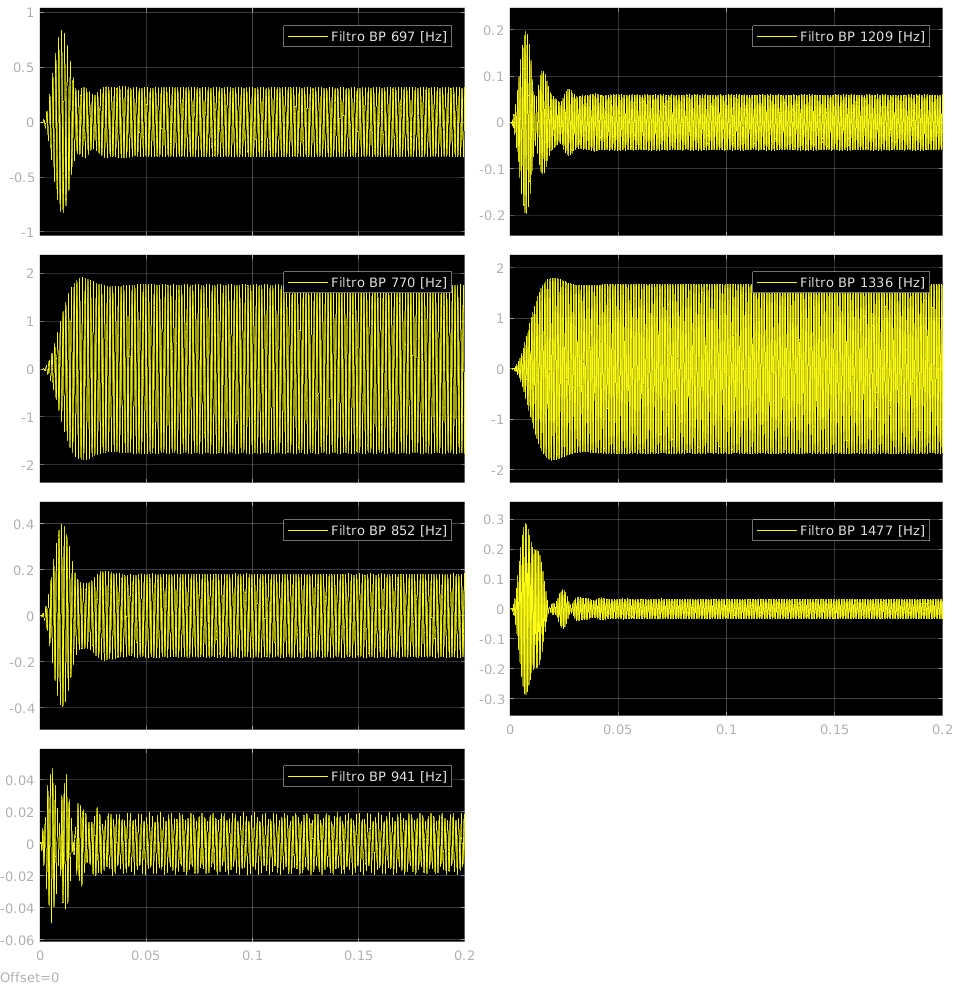
\includegraphics[width=\linewidth]{images/simulacion/fallas/bank/5.png}
  \caption{Señales en el Banco de Filtro}
  \label{fig:num_5_bank}
\end{figure}

\begin{figure}[H]
  \centering
  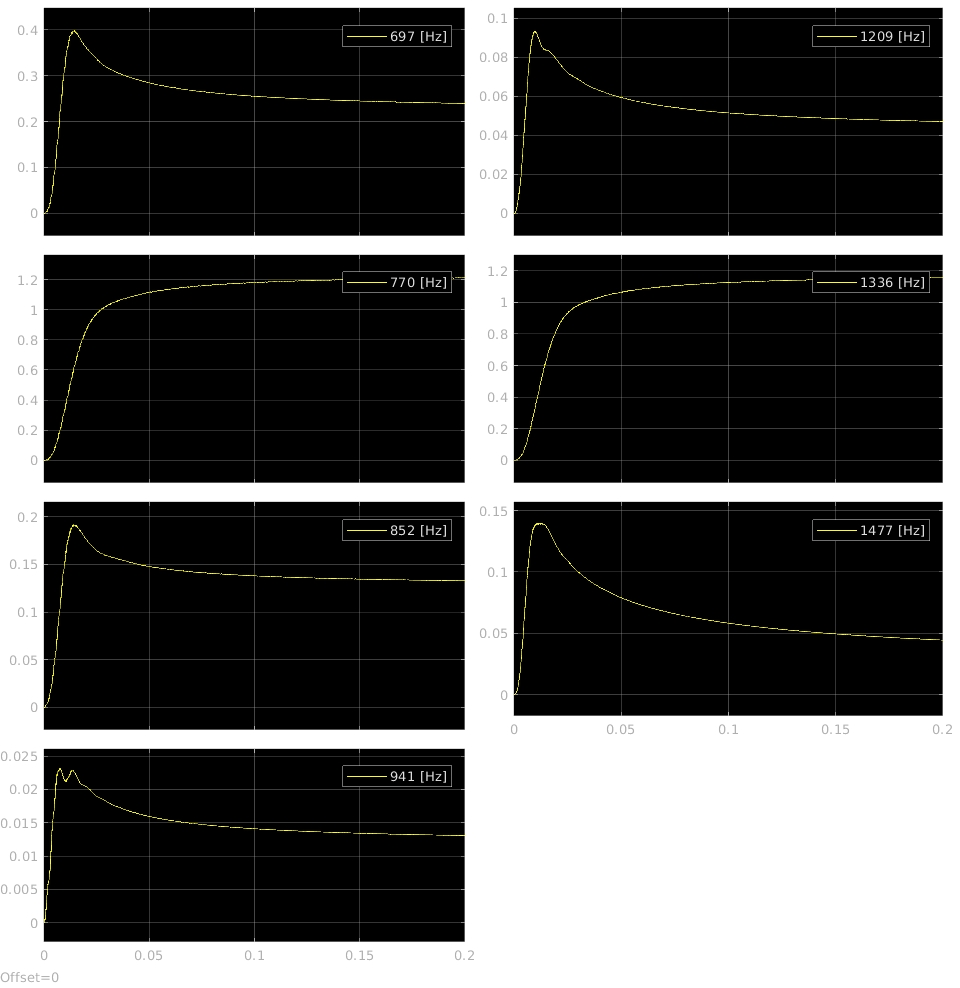
\includegraphics[width=\linewidth]{images/simulacion/fallas/rms/5.png}
  \caption{Valor Eficaz de las salida del Banco de Filtros }
  \label{fig:num_5_rms}
\end{figure}

Ya que ambos valores eficaces de las señales que codifican la Tecla 5 son mayores a 1, se reconoce la activación de la misma.

% ******************************************************* %

\section{Número 6: 770 [Hz] + 1477 [Hz]}
\label{sec:signal_6}
\begin{figure}[H]
  \centering
  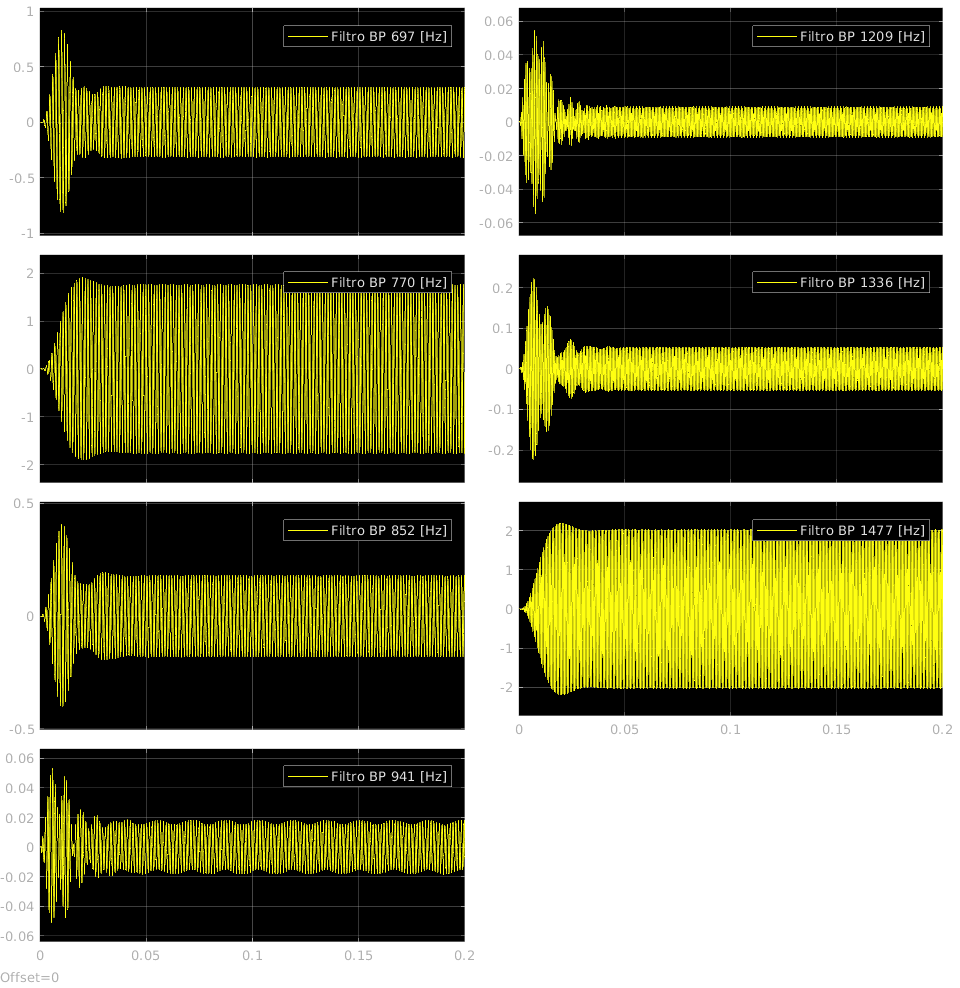
\includegraphics[width=\linewidth]{images/simulacion/fallas/bank/6.png}
  \caption{Señales en el Banco de Filtro}
  \label{fig:num_6_bank}
\end{figure}

\begin{figure}[H]
  \centering
  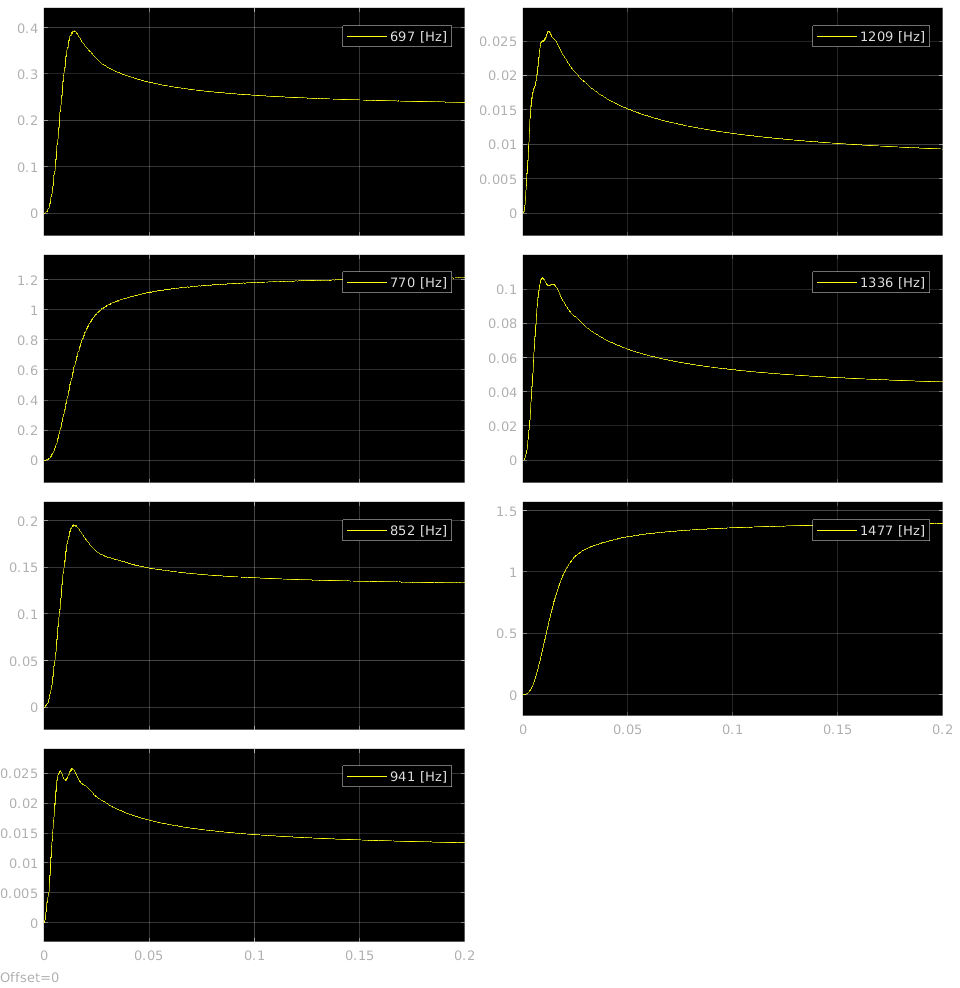
\includegraphics[width=\linewidth]{images/simulacion/fallas/rms/6.png}
  \caption{Valor Eficaz de las salida del Banco de Filtros }
  \label{fig:num_6_rms}
\end{figure}

Ya que ambos valores eficaces de las señales que codifican la Tecla 6 son mayores a 1, se reconoce la activación de la misma.

% ******************************************************* %

\section{Número 7: 852 [Hz] + 1209 [Hz]}
\label{sec:signal_7}
\begin{figure}[H]
  \centering
  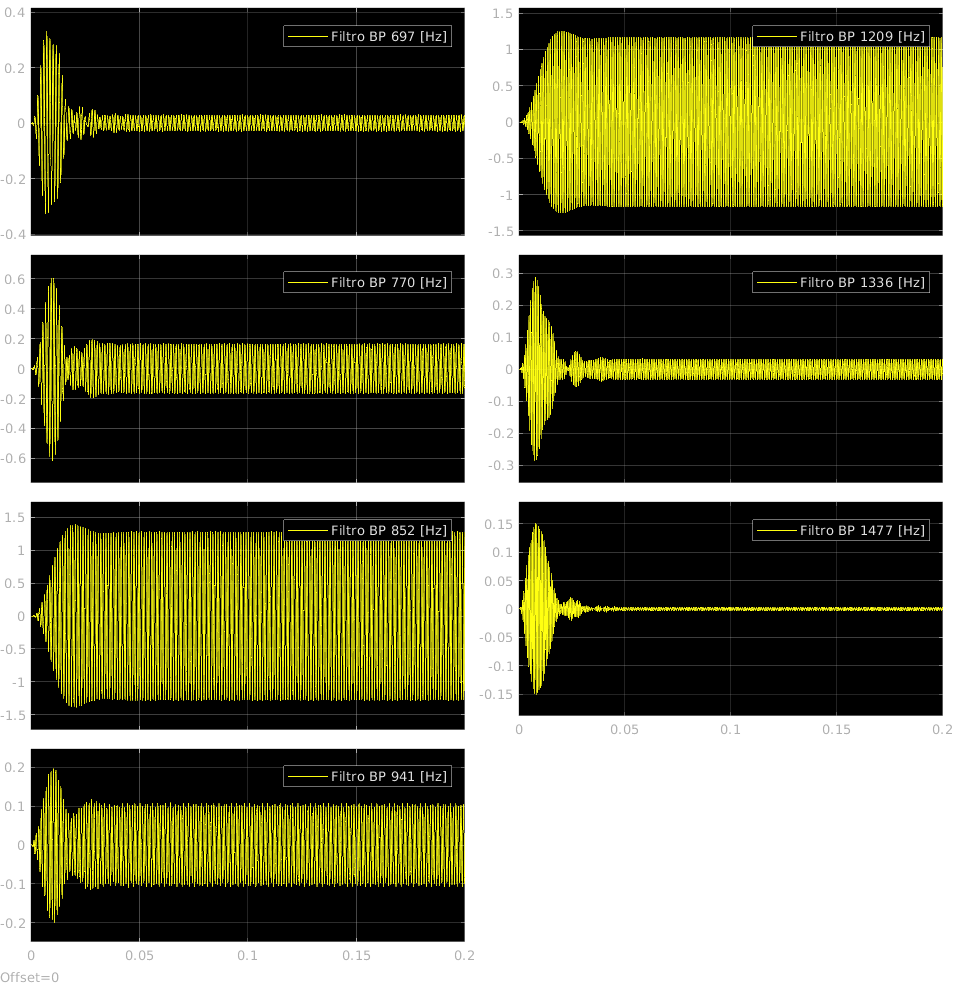
\includegraphics[width=\linewidth]{images/simulacion/fallas/bank/7.png}
  \caption{Señales en el Banco de Filtro}
  \label{fig:num_7_bank}
\end{figure}

\begin{figure}[H]
  \centering
  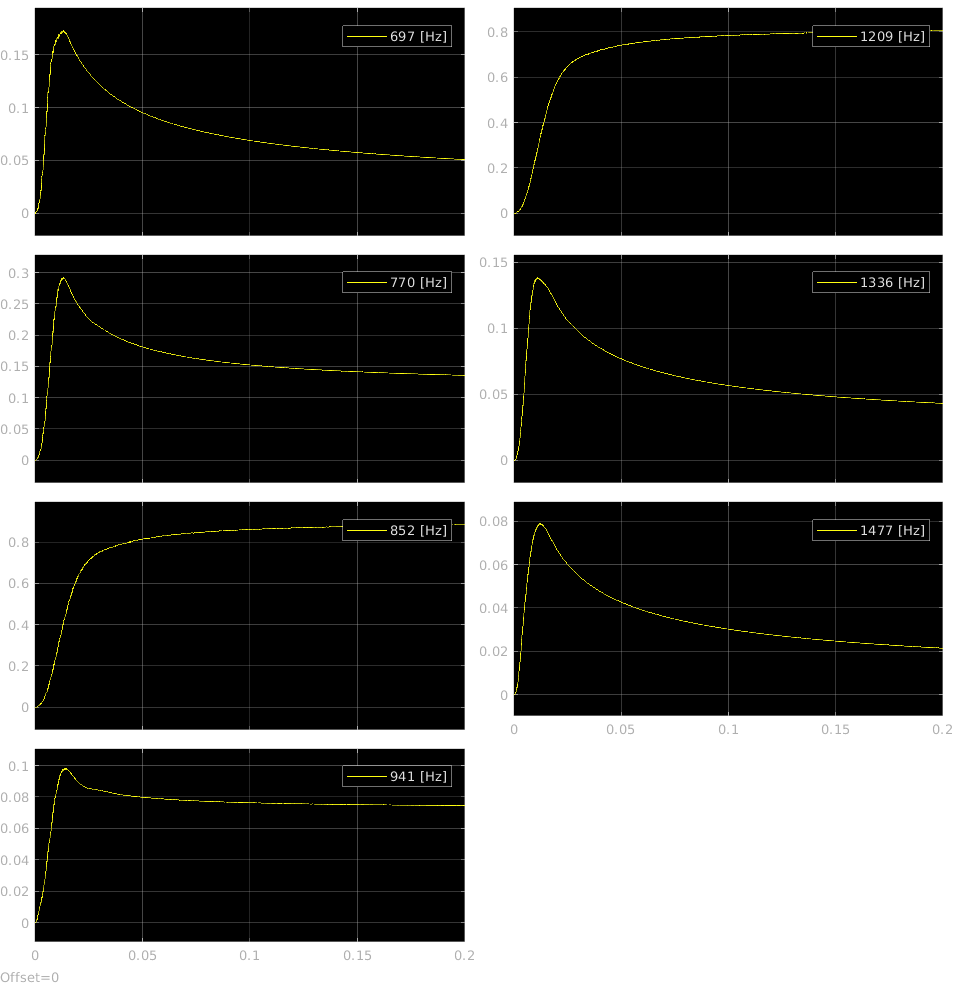
\includegraphics[width=\linewidth]{images/simulacion/fallas/rms/7.png}
  \caption{Valor Eficaz de las salida del Banco de Filtros }
  \label{fig:num_7_rms}
\end{figure}

Debido a que los valores eficaces de las señales que codifican a la Tecla 7 son menores a 1, estas se toman como 0 para la compuerta lógica. En consecuencia, no se reconoce la activación de la misma.

% ******************************************************* %

\section{Número 8: 852 [Hz] + 1336 [Hz]}
\label{sec:signal_8}
\begin{figure}[H]
  \centering
  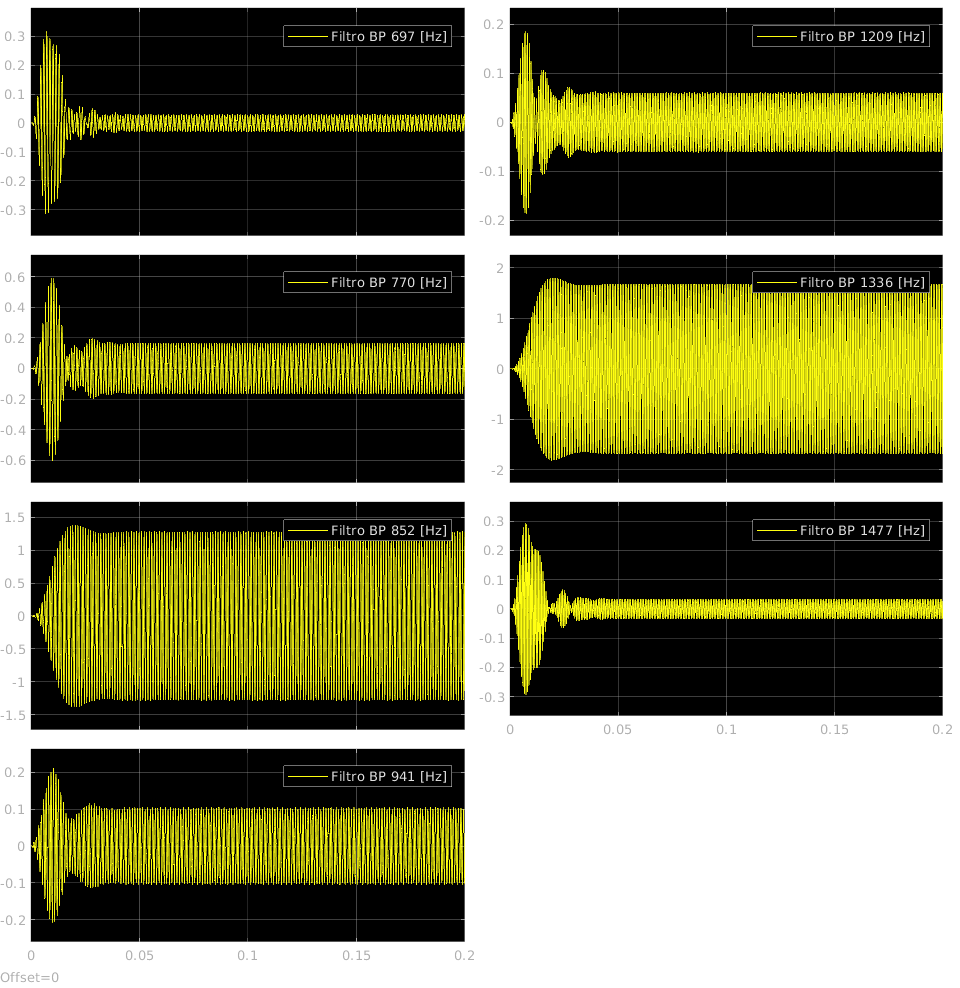
\includegraphics[width=\linewidth]{images/simulacion/fallas/bank/8.png}
  \caption{Señales en el Banco de Filtro}
  \label{fig:num_8_bank}
\end{figure}

\begin{figure}[H]
  \centering
  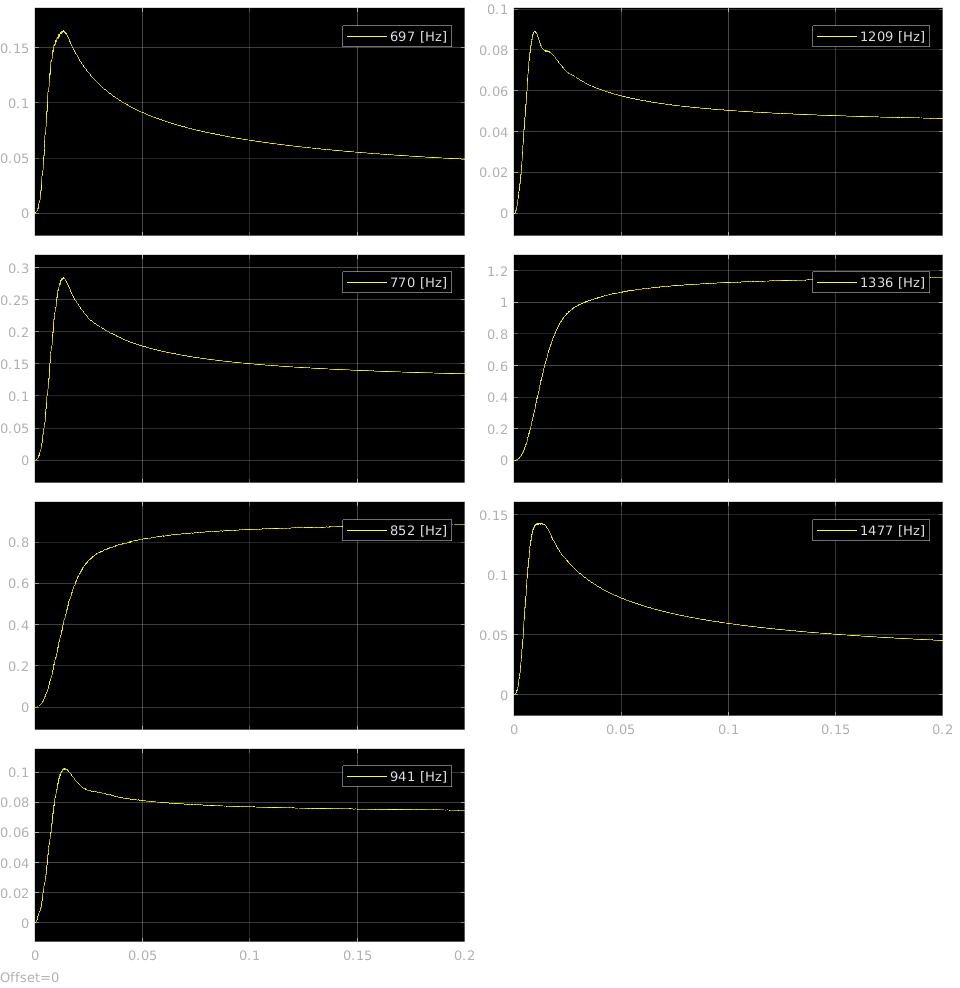
\includegraphics[width=\linewidth]{images/simulacion/fallas/rms/8.png}
  \caption{Valor Eficaz de las salida del Banco de Filtros }
  \label{fig:num_8_rms}
\end{figure}

Debido a que el valor eficaz de la señal del filtro de 852 [Hz] es menor a 1, esta se toma como 0 para la compuerta lógica. En consecuencia, no se reconoce la activación de la Tecla 8.

% ******************************************************* %

\section{Número 9: 852 [Hz] + 1477 [Hz]}
\label{sec:signal_9}
\begin{figure}[H]
  \centering
  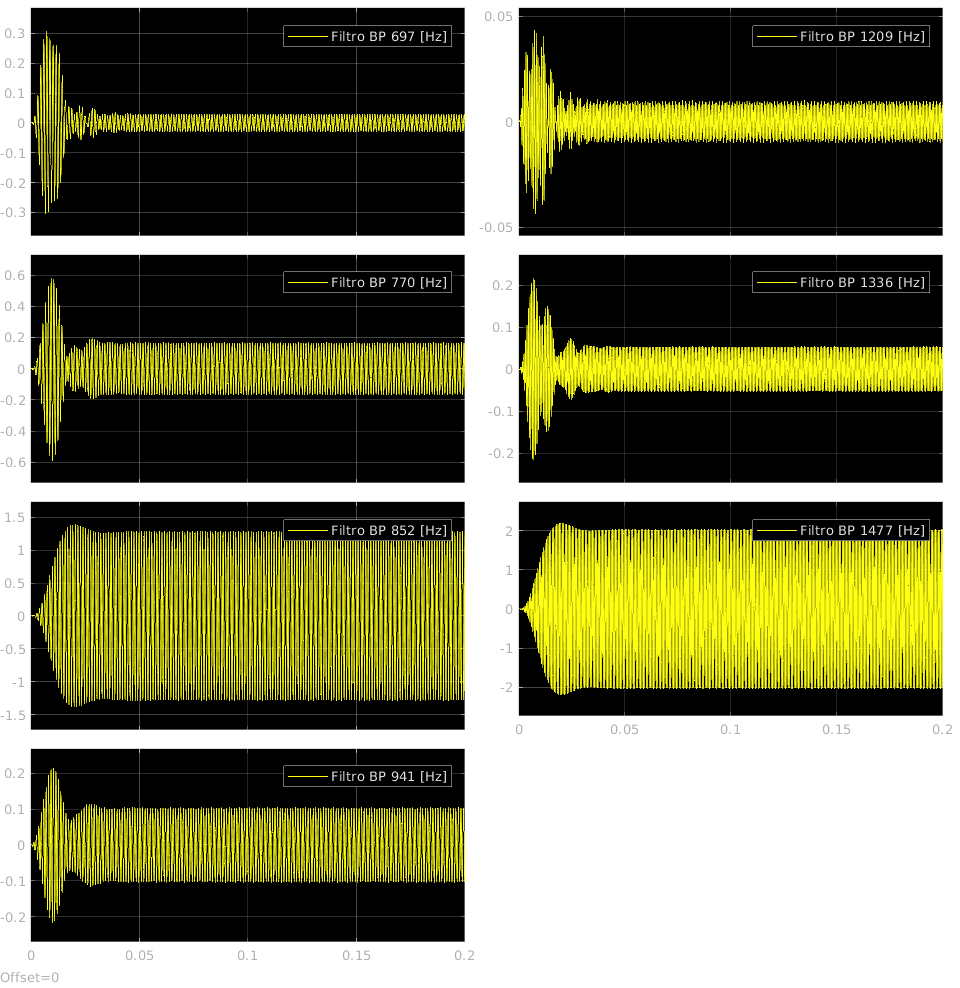
\includegraphics[width=\linewidth]{images/simulacion/fallas/bank/9.png}
  \caption{Señales en el Banco de Filtro}
  \label{fig:num_9_bank}
\end{figure}

\begin{figure}[H]
  \centering
  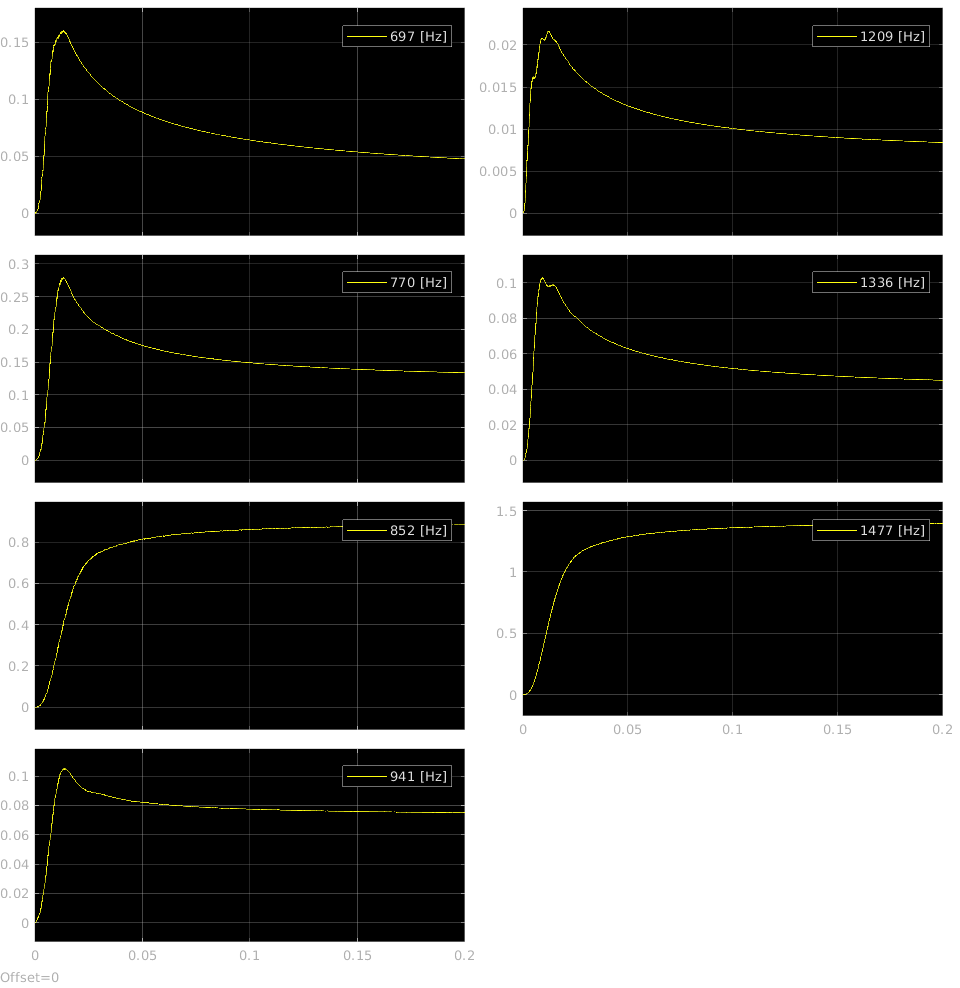
\includegraphics[width=\linewidth]{images/simulacion/fallas/rms/9.png}
  \caption{Valor Eficaz de las salida del Banco de Filtros }
  \label{fig:num_9_rms}
\end{figure}

Debido a que el valor eficaz de la señal del filtro de 852 [Hz] es menor a 1, esta se toma como 0 para la compuerta lógica. En consecuencia, no se reconoce la activación de la Tecla 9.

% ******************************************************* %

\section{Número 0: 941 [Hz] + 1336 [Hz]}
\label{sec:signal_0}
\begin{figure}[H]
  \centering
  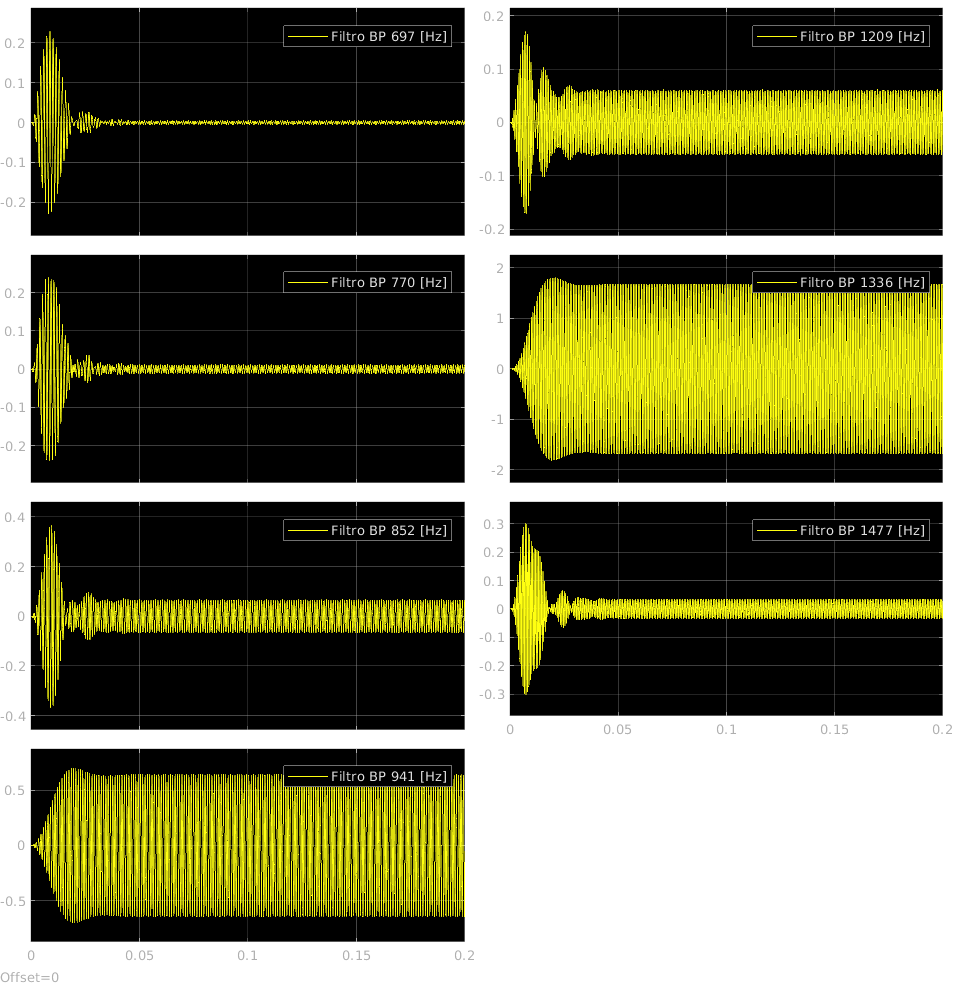
\includegraphics[width=\linewidth]{images/simulacion/fallas/bank/0.png}
  \caption{Señales en el Banco de Filtro}
  \label{fig:num_0_bank}
\end{figure}

\begin{figure}[H]
  \centering
  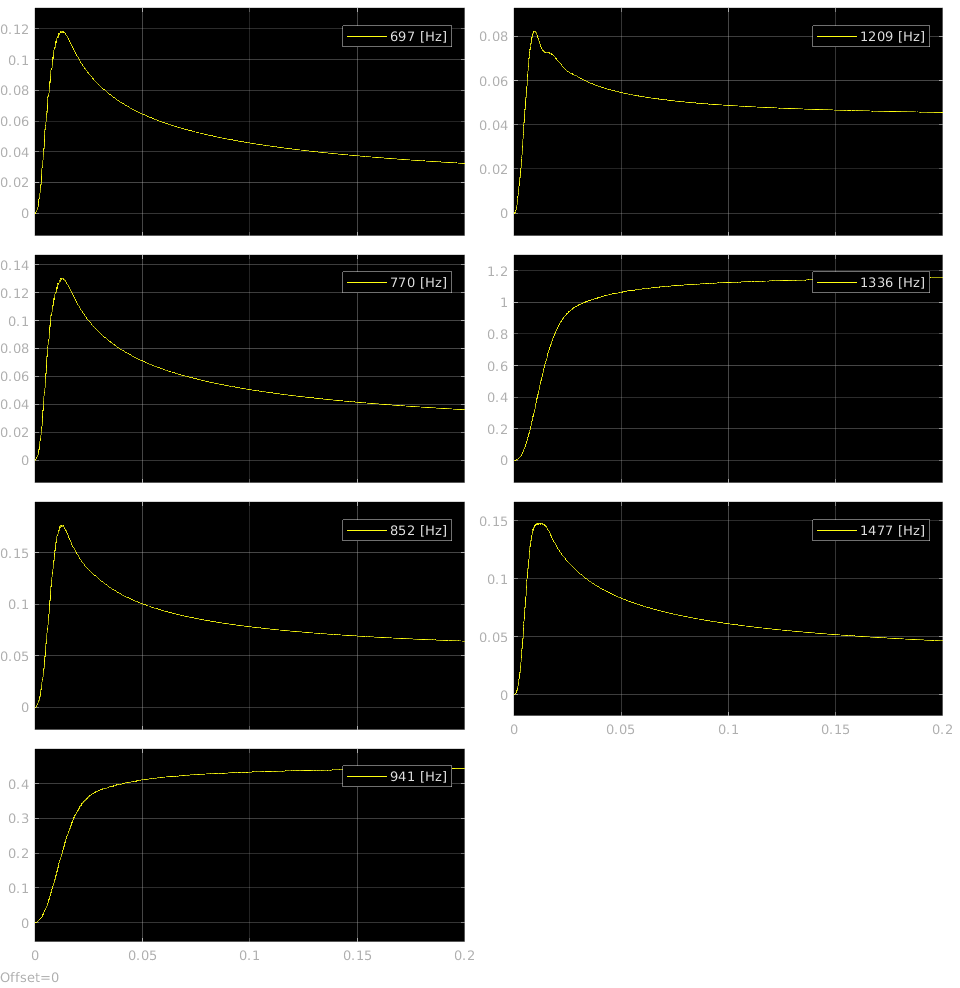
\includegraphics[width=\linewidth]{images/simulacion/fallas/rms/0.png}
  \caption{Valor Eficaz de las salida del Banco de Filtros }
  \label{fig:num_0_rms}
\end{figure}

Debido a que el valor eficaz de la señal del filtro de 941 [Hz] es menor a 1, esta se toma como 0 para la compuerta lógica. En consecuencia, no se reconoce la activación de la Tecla 0.
